\documentclass{scrreprt}
\usepackage{graphicx}
\usepackage{tabularx}
\usepackage{listings}
\usepackage{underscore}
\usepackage[bookmarks=true]{hyperref}
\usepackage[utf8]{inputenc}
\usepackage[english]{babel}
\usepackage[margin=2cm]{geometry}
\textheight = 690pt
\headheight = 27pt

\hypersetup{
bookmarks=false, % show bookmarks bar?
pdftitle={RSA, projet MyAdBlock}, % title
pdfauthor={RUCHOT Guillaume, MOLLARD Romaric}, % author
pdfsubject={RSA - Réseau Avancé, projet MyAdBlock}, % subject of the document
pdfkeywords={proxy, c, network, adblock, socket, tcp}, % list of keywords
colorlinks=true, % false: boxed links; true: colored links
linkcolor=black, % color of internal links
citecolor=black, % color of links to bibliography
filecolor=black, % color of file links
urlcolor=blue, % color of external links
linktoc=page % only page is linked
}%


%\renewcommand{\familydefault}{\sfdefault}
\renewcommand*{\chapterheadstartvskip}{\vspace*{0cm}}
\renewcommand*{\chapterheadendvskip}{\vspace{1cm}}
\def\myversion{1.0}
\date{}
\usepackage{hyperref}

\addto\captionsenglish{%
\renewcommand\contentsname{Sommaire}%
}

\def\nbpage{9}

\def\code#1{\texttt{#1}}
\let\tab\quad
\usepackage{fancyhdr}
\pagestyle{fancy}
\fancyhead[L]{RSA Réseau, Projet MyAdBlock}
\fancyhead[R]{\leftmark}
\fancyfoot[L]{Télécom Nancy, Avril 2017}
\fancyfoot[C]{}
\fancyfoot[R]{\thepage\ sur \nbpage}
\fancypagestyle{plain}{%
\fancyhead[L]{RSA Réseau, MyAdBlock}
\fancyhead[R]{\leftmark}
\fancyfoot[L]{Télécom Nancy, Avril 2017}
\fancyfoot[C]{}
\fancyfoot[R]{\thepage\ sur \nbpage}
}
\renewcommand{\headrulewidth}{0pt}

\begin{document}

\thispagestyle{empty}
\begin{bfseries}
\begin{figure}

\includegraphics[height=1.8cm]{images/tn.png}
\hspace{1.2cm}

\includegraphics[height=1.8cm]{images/ul.png}
\vspace{3cm}
\end{figure}
\begin{flushright}
\rule{\paperwidth}{1pt}
\\
\vspace{2cm}
\Huge{RSA - Réseau Avancé}\\
\vspace{0.5cm}
\huge
Projet MyAdBlock\\
\vspace{1.9cm}
\Large
\vspace*{\fill}
RUCHOT Guillaume\\
MOLLARD Romaric\\
\vspace{1.9cm}
\small
Avril 2017\\
\end{flushright}
\end{bfseries}

\tableofcontents
\clearpage

\clearpage
\setcounter{page}{1}

\chapter{Introduction}

\section{À propos de ce document}
Ce document a pour but de présenter le projet \textit{MyAdBlock} et son élaboration. Le projet \textit{MyAdBlock} consiste en la réalisation d'un proxy HTTP/HTTPS capable de bloquer les accès à certains sites en utilisant une liste spécifique de masques, dans le but par exemple de bloquer les publicités.
Ce projet a été réalisé dans le cadre de l'étude de l'utilisation avancée du système et du réseau du niveau application au niveau transport. Le langage utilisé est le C, pour sa proximité avec le système.\\
Créer un serveur de ce type permet de comprendre pleinement le fonctionnement TCP pour le transport du protocole HTTP : les information contenues dans les entêtes HTTP, la transformation des nom de serveurs en adresses, l'obligation pour le serveur d'avoir une gestion simultanée des clients...\\

\section{Remerciements}
Nous avons réalisé ce projet à l'aide des sources suivantes :\\\\
\textbf{Documentation linux (ici getaddrinfo(3))}\\
http://man7.org/linux/man-pages/man3/getaddrinfo.3.html\\
\\
\textbf{Wireshark}\\
https://www.wireshark.org/\\
\\
\textbf{Liste de filtres publicitaires}\\
http://easylist.to/\\
\\
\textbf{Conversion nom de domaine vers adresse ip}\\
http://get-site-ip.com/\\

\chapter{Partie I - Étude du fonctionnement}

\section{Observation du dialogue navigateur/serveur}

Nous utiliserons pour la suite deux navigateurs, Firefox qui sera configuré pour fonctionner avec un proxy local sur le port 80, et Chrome qui lui permettra de comparer les résultats.

\subsection{Observation avec wireshark}

Nous avons commencé par observer les transmissions TCP entre Chrome et www.telecomnancy.eu avec Wireshark. Comme www.telecomnancy.eu renvoie une redirection HTTP 301, nous avons filtré les résultats sur l'adresse ip 193.50.135.38, qui correspond à l'adresse ip du serveur telecomnancy.univ-lorraine.fr.
\\
Ainsi le filtre WireShark devient celui-ci :
ip.dst_host == 193.50.135.38 or ip.src_host == 193.50.135.38

\begin{center}
  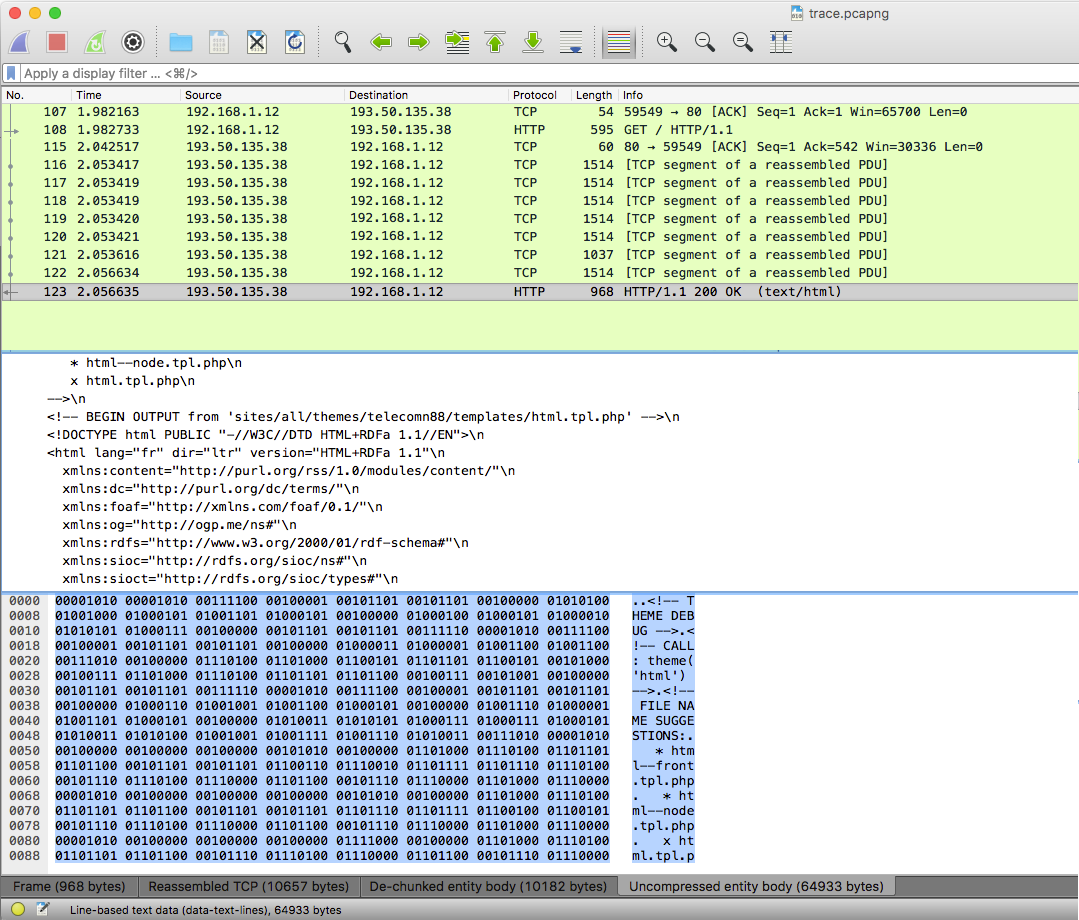
\includegraphics[height=7.5cm]{images/f1.png}
  \\
  \textit{Figure 1 : Trace Wireshark contenant la communication vers telecomnancy.univ-lorraine.fr}
\end{center}


Pour observer le contenu HTTP d’une transmission, il faut regarder le tout dernier élément de la transmission (ici l'élément 123, HTTP 200 OK, figure 1), et demander à Wireshark de décompresser le contenu. Le document html est compressé, et ainsi on ne peut pas travailler dessus tant qu’il n’est pas complet. Cependant, le header HTTP n'est jamais compressé, ni pour l'envoi ni pour la réponse, et ce pour permettre au navigateur d'obtenir des informations comme la taille du contenu en cours de reception (content-length).\\\\

Nous remarquons que la communication commence par l'envoi d'un paquet TCP contenant la requette HTTP "GET" (élément 108, figure 1, les lignes précédentes concernent la mise en place de la connexion TCP), suivi du contenu de la page envoyé en retour. Le tout se fait via TCP.\\
En regardant les paquets TCP en détail, nous remarquons que le dernier paquet envoyé possède le flag FIN, et c'est le seul élément nous permettant à priori d'obtenir l'information de fin de transmission.\\\\

Nous pouvons noter que le protocole HTTP ne contient pas l'ip du serveur distant et seulement le nom du serveur.

\subsection{Observation avec wireshark après mise en place du proxy}
Nous avons configuré Firefox pour se connecter à un serveur proxy local qui n'est qu'un simple serveur TCP basique (qui accepte les connexions) afin d'observer le comportement de Firefox et surtout les informations envoyées au futur proxy.\\
Dans ce cas nous devons observer les transactions locales dans le mode "Loopback Io0".

\begin{center}
  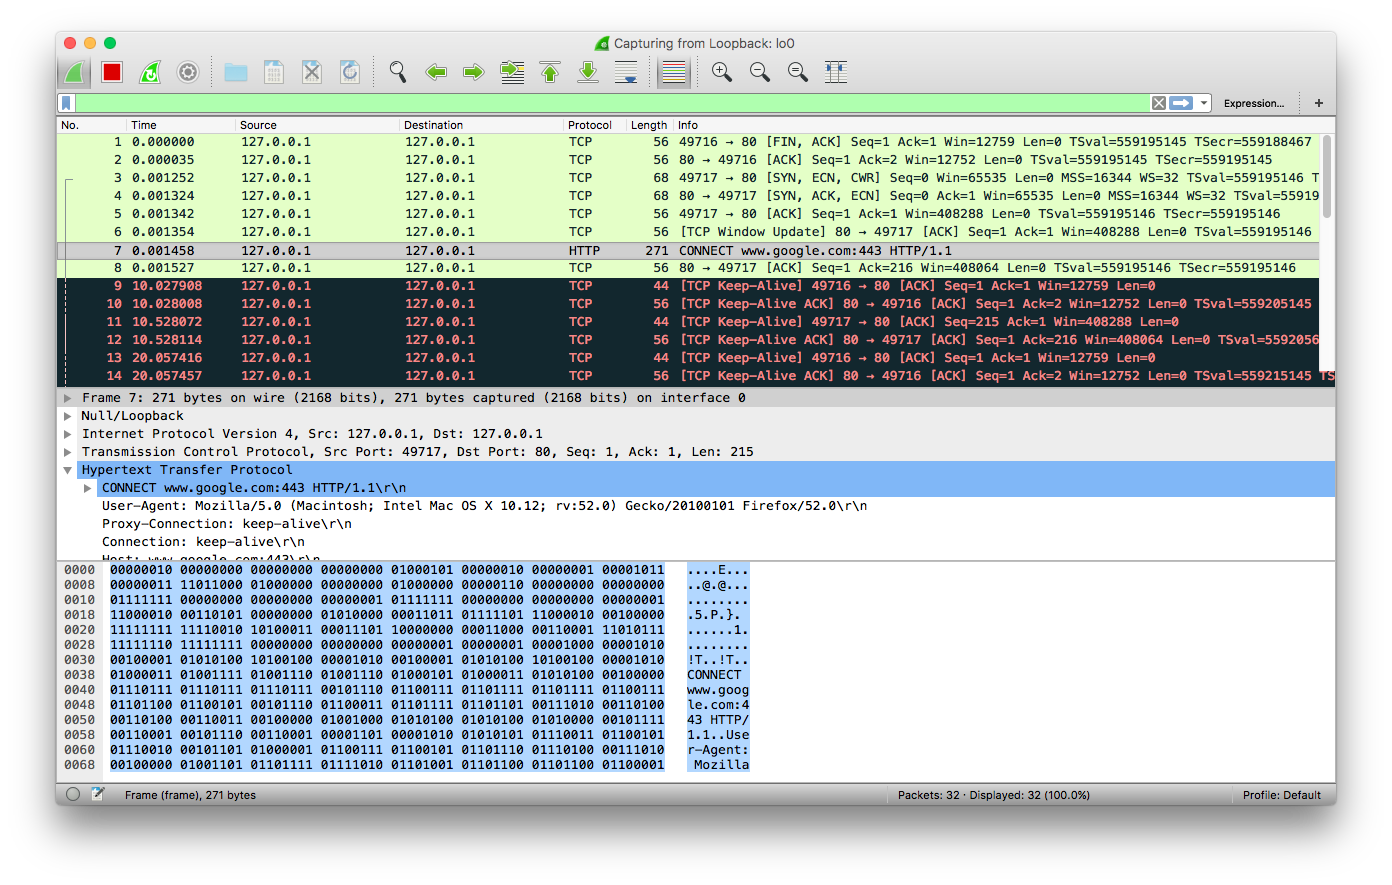
\includegraphics[height=7.5cm]{images/f2.png}
  \\
  \textit{Figure 2 : Trace Wireshark contenant la communication vers telecomnancy.univ-lorraine.fr avec proxy}
\end{center}

Nous observons ici qu'après la connexion TCP, Firefox envoie le header HTTP "CONNECT" (qui est un équivalent de GET dans le cas du https) au proxy local (ligne 7 de la figure 2). En observant le contenu de cette entête nous confirmons que nous n'avons aucun moyen de connaitre directement par lecture l'adresse ip du serveur web demandé. Nous devrons donc utiliser des outils comme gethostbyname(1) ou getaddrinfo(3).

\subsection{Observation avec un serveur TCP de base}
En mettant en place un serveur TCP très basique étudié en cours, nous avons remarqué que les navigateurs ouvraient une nouvelle connexion au serveur pour chaque url voulue. La question de la gestion simultanée de plusieurs clients est donc primordiale si nous voulons qu'une page web ne charge pas chaque composant (js, css, iframes...) un par un.

\section{Spécification du proxy MyAdBlock}
Après les observations effectuées sur WireShark, nous avons mis en place le fonctionnement général de notre programme.\\
Nous avons séparé la réalisation du projet en plusieurs étapes.

\subsection{Création d'un proxy HTTP transparent}
Dans un premier temps, une grande partie du travail était la réalisation d'un proxy permettant l'accès à internet. Si ceci semble simple en apparence, c'est la partie la plus importante du travail dans ce projet. Internet évolue très rapidement et si nous développions un proxy limité à l'IPv4 et le protocole HTTP, nous ne pourrions pas afficher grand chose. Nous avons donc décidé de mettre en place notre proxy transparent en commencant de manière simple sur cette url :\\
http://www.example.com/\\
Son contenu est très court (tient en un seul paquet en temps normal), l'accès se fait via HTTP (pas de HTTPS) et enfin il n'y a pas de liens internes, c'est à dire que le navigateur ne va pas chercher d'autres liens pour charger des images par exemple ou des feuilles de style css.\\
Afin d'étendre notre proxy à la réception de plusieurs paquets réponse et la connexion de clients multiples, nous avons utilisé un autre site web simple :\\
http://cheval.fr/\\
Celui-ci contient une image, qui ne tient pas en un seul paquet, ce qui permet de vérifier un autre point du proxy.

\subsection{Prise en compte des connexions HTTPS}
Il est presque impossible d'utiliser internet sans le protocole HTTPS, car même les sites web HTTP utilisent des publicités externes ou bien des feuilles de styles générales (bootstrap) accéssibles seulement via HTTPS.\\
Heureusement détecter les transactions SSL est simple puisqu'il suffit de détecter la méthode "CONNECT".
\\
Nous testerons cette fonctionnalité simplement sur google et sur\\
https://www.leboncoin.fr

\subsection{Filtrage des URL}
Nous effectuerons le filtrage des accès sur le second argument des entêtes HTTP, soit le chemin demandé. Il contient à quelques détails près l'url visible dans le navigateur.\\
Le programme génèrera une LinkedList contenant l'intégralité des masques à utiliser. Lorsqu'une nouvelle url sera demandée, si l'un de ces masques est entièrement contenu dans cette url alors l'url est refusée.

\subsection{Résumé}
Voici un résumé graphique du fonctionnement du proxy MyAdBlock.

\begin{center}
  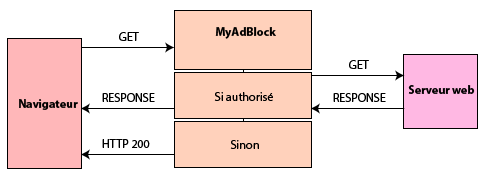
\includegraphics[height=4.5cm]{images/f3.png}
  \\
  \textit{Figure 3 : Fonctionnement de MyAdBlock}
\end{center}


\section{Recherche de masques et filtres pour la publicité}
Pour tester une des utilisations du proxy qui est le filtrage des publicité, nous avons utilisé les listes présentes sur le site :\\
http://easylist.to/\\
Une bonne partie de cette liste concerne des éléments du contenu HTML d'un site web, nous ne pouvons pas utiliser ces éléments car nous n'avons à aucun moment accès au contenu brut des pages transférées.

\chapter{Partie II - Création de l'outil}

\section{Fonctionnement général du programme}
Le programme fonctionne en N parties.

\subsection{Démarrage du serveur principal d'écoute des clients}

Tout d'abord, nous récupérons les options demandées par le client à l'aide de la fonction getopt. Ensuite, soit nous affichons le manuel d'aide s'il nous est demandé, soit nous passons à la création du serveur:\\
Pour le serveur et toutes les communications que nous faisons avec ce proxy, nous nous servons des socket tels que nous les avons vus en cours de RSA.\\
Ainsi nous lions un socket d'écoute à un port (par default le port 80) sur lequel le navigateur du client pourra se connecter.\\
Ensuite nous pouvons lancer la boucle principale d'écoute pour les clients. Celle-ci se chargera de récupérer toutes les requêtes arrivant depuis le port défini sur l'adresse localhost (127.0.0.1).\\
Lorsqu'une requête arrive, le programme se dédouble grâce à la fonction \code{fork()} et nous passons à l'étape suivante.

\subsection{Lecture du header}

Pour simplifier les fonctions suivantes du programme, nous chargeons les différentes données disponibles dans une structure header dont le schéma est le suivant :\\
\\
\code{
  struct header {\\
  \tab  char ssl; //1 si c'est une connexion HTTPS\\
  \tab  char method[500]; //GET, CONNECT, POST...\\
  \tab  char path[500]; //Chemin demandé\\
  \tab  char protocol[500]; //HTTP/1.1 par exemple\\
  \tab  char hostname[500]; //Nom du domaine\\
  \tab  struct host hst; //Données calculées selon le nom de domaine pour obtenir une adresse réelle sur le réseau.\\
  };\\
  struct host {\\
  \tab  int port; //Port\\
  \tab  int addr_family; //Type d'adresse (AF_INET pour IPv4, AF_INET6 pour IPv6)\\
  \tab  int addr_len;\\
  \tab  struct sockaddr_in6 addr;\\
  };\\
}
\\
Pour commencer, les premières données se trouvent dans la première ligne de l'entête HTTP qui est de la forme\\
\code{METHODE URLPATH PROTOCOLE},\\
Par exemple :\\
\code{GET https://www.wireshark.org/lists/ HTTP/1.1}\\
\\
Nous décomposons les différents morceaux de cette première ligne à l'aide de la fonction \code{strchr(2)} qui nous renvoie la position du prochain caractère demandé (ici espace).\\
Ensuite, les autres données sont disponibles sous la forme :\\
Clé: valeur\\
Nous avons donc créé une fonction qui recherche une valeur en fonction d'une clé, sous ce format précis. Ainsi nous récupérons la donnée très importante associée à la clé "Host: ". Cette valeur n'est rien d'autre que le domaine avec le quel nous devrons communiquer.\\
\\
Il reste alors le champ \code{hst} à remplir, qui contiendra une véritable adresse IPv4 ou IPv6. Nous utilisons la fonction \code{getaddrinfo(3)} et récupérons de préférence une adresse IPv4 parmis les résultats retournés (cette fonction retourne une liste d'adresses correspondantes). Sinon nous prenons la version IPv6 si aucune version IPv4 n'est disponible.

\subsection{Filtrage}
Avant de démarrer le proxy, nous chargeons les fichiers filtres donnés en paramètres, chaque masque (et donc chaque ligne) est chargé dans une linked liste.\\
Une fois que nous avons l'entête utilisable, nous pouvons effectuer un filtrage par exemple sur le paramètre \code{path}, qui contient le plus d'information utile sur l'URL. Nous regardons alors pour chaque élément de la précédente liste si cet élément est entièrement contenu dans l'url donnée.\\
Si c'est le cas, alors nous considérons que nous avons une publicité et nous renvoyons une réponse vide et valide (HTTP 200 OK).


\subsection{Communication en HTTP}

Lorsque l'on détecte une demande http vers un serveur non bloqué, on crée un socket de dialogue vers ce navigateur (en lui envoyant la requête), et nous traitons son retour de manière détaillée:\\
Tout d'abord, nous lisons (et envoyons au client) le header html de la réponse du serveur ligne par ligne (à l'aide de la fonction \code{fgets()}) pour essayer d'y détecter le champ "Content-Lenght". Ce champ, dont la présence n'est pas obligatoire, nous indique par avance la taille du message attendu.\\\\
Ensuite, nous lisons et envoyons au client le message caractère par caractère, en s'arrêtant lorsque l'on détecte un caractère EOF, ou lorsque l'on atteint la taille du message indiquée dans le header.\\
Notre manière d'envoyer les données au client peut sembler être une immense perte de temps, mais ce n'est pas le cas car nous appliquons (ou du moins nous ne désactivons pas) l'algorithme de Naggle. Ainsi, même si l'on demande l'envoi de messages de 1 octet, ces derniers seront regroupés avant d'être envoyés au navigateur du client.\\
Une fois la communication terminée, nous fermons les sockets de dialogue avec le client et le serveur, avant de terminer le processus qui se chargeait de la communication.
\subsection{Communication en SSL}

La communication en SSL (https) est différente de la communication en http car elle assure que le transport des données est complètement confidentiel, et que l'on ne peut pas lire le contenu des paquet sur le chemin (comme nous le faisons pour la communication http).\\ Le fonctionnement général de SSL est le suivant : \\
Deux hôtes qui veulent se connecter vont d'abord s'accorder sur les clés de sécurité, version, ... C'est ce qu'on appelle le "handshake". Ensuite ces deux hôtes communiquent de manière totalement cryptée, et enfin ils peuvent vérifier des informations sur la communication après coup.\\
\\
Ainsi, nous avions deux choix :\\
- Le premier était de créer un véritable serveur acceptant les connexion SSL du client, récupérant ses requêtes, et les relayant au serveur externe en se connectant à lui en SSL. Mais cela aurait allongé considérablement le temps de dialogue et il nous aurait fallu obtenir une PKI.\\
- La seconde, que nous avons choisi, était de simplement faire office de tunnel pour la connexion SSL. C'est à dire que lorsque nous recevons un message du client, nous l'envoyons immédiatement au serveur distant, et vice-versa. Le problème causé par cette solution est que nous ne pouvons pas toujours connaître la terminaison de la discussion entre le serveur et le client, ainsi nous avons mis en place un mécanisme de timeout qui rompt la connexion au bout de 4 secondes sans réponse. Ceci nous permet aussi d'éviter d'attendre trop longtemps la réponse d'un serveur qui ne serait pas fonctionnel.

\subsection{Résultat}

Comme nous pouvons le voir sur l'image suivante, nous filtrons avec succès la publicité présente sur le site leboncoin.fr.
\\
\begin{center}
  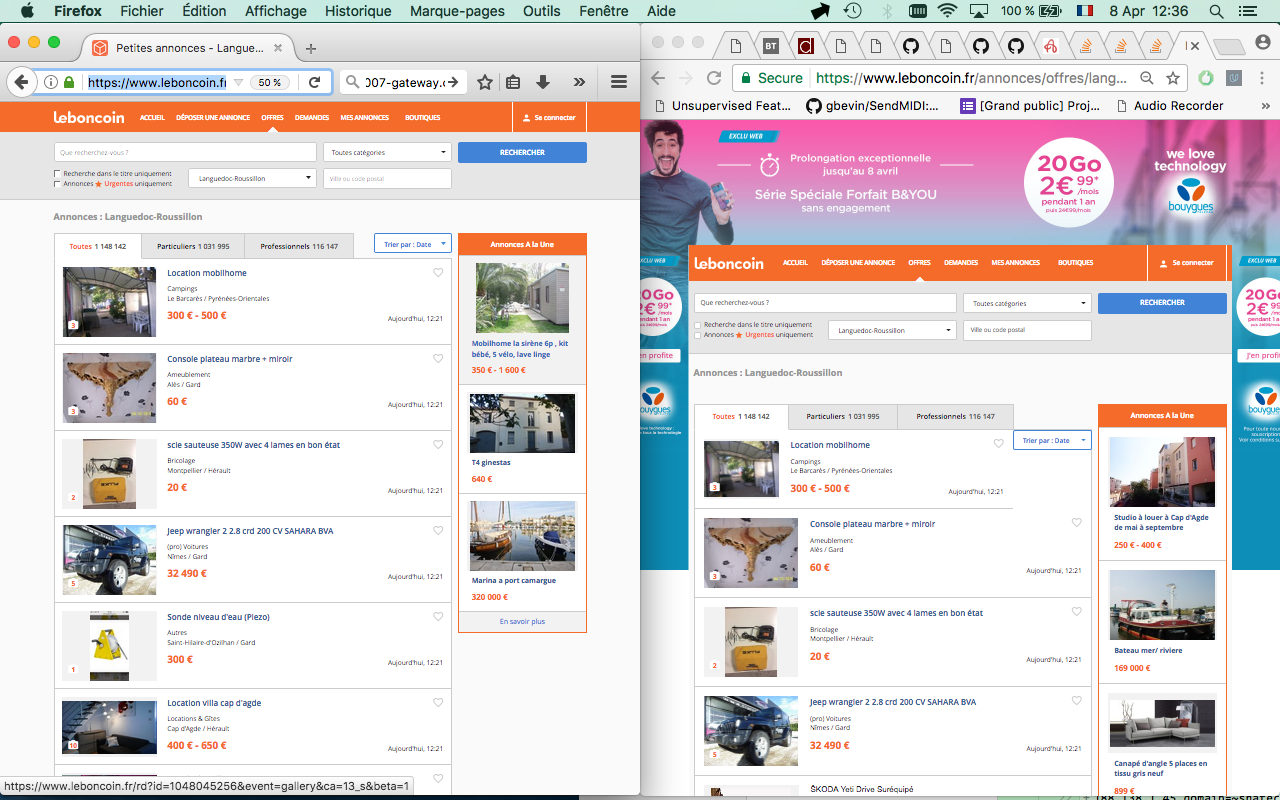
\includegraphics[height=7.5cm]{images/f4.png}
  \\
  \textit{Figure 4 : À gauche Firefox utilisant le proxy, à droite Chrome sans proxy.}
\end{center}

\section{Difficultés rencontrées}

\subsection{Détection de la fin des transmissions}
Dans un premier temps, nous nous attendions simplement à recevoir un message vide pour indiquer la fin des données transmises, cependant ce ne fut pas le cas, et bien que la page fut chargée entièrement, le navigateur continuait d'attendre la fin du chargement. \\
De plus, la structure que nous utilisons pour faire nos communication (les sockets) se situent juste au dessus de TCP, et ainsi on ne peut pas récupérer les flags de ce protocole (le flag FIN aurait pu ici nous servir).\\
Ainsi, la seule solution que nous ayons trouvé a été d'envoyer le message caractère par caractère jusqu'à la fin du message (signifiée soit par un EOF, soit lorsque l'on arrive au nombre de caractères s'il est spécifié dans le header html).

\subsection{Plusieurs paquets du navigateur}
Nous pensions à tort que l'entête HTTP était envoyée dans un seul paquet. Nous analysions et relayions ce paquet sans nous poser plus de questions. Cependant en allant sur le site de publicité http://01.net, nous avons très vite remarqué que les fervants utilisateurs de Cookies envoyaient de très lourds paquets aux serveurs.\\
Nous avons donc édité le code pour envoyer chaque morceaux comme nous le faisons dans l'autre sens pour la réception des pages web.

\subsection{Préparation à l'IPv6}
Dans un premier temps, nous avons utilisé \code{gethostbyname(1)} pour obtenir une adresse IPv4 correspondant à un nom de domaine. Cependant il fallait prendre en compte l'utilisation des adresses IPv6 qui commencent à être de plus en plus utilisées sur Internet.\\
Pour celà nous avons utilisé \code{getaddrinfo(3)} qui prend en argument le nom de domaine et le port. La modification du code ne s'est pas faite facilement, et c'est en étudiant d'autres codes et comparant plusieurs documentations que nous avons compris que nous pouvions caster les structures prévues pour l'IPv4 et celles pour l'IPv6 afin de les rendre compréhensibles par la fonction \code{socket(4)}.

\section{Limites et améliorations du programme}
Pour le moment le filtrage des url se fait après la recherche de l'adresse associée au nom de domaine, ce qui utilise légèrement le réseau alors que nous allons ignorer la réponse.\\
\\
Nous ne sommes pas capables d'éditer directement le code HTML retourné car il est souvent compressé ou crypté dans le cas d'une connexion HTTPS. Nous sommes alors très limité car nous utilisons seulement les données disponibles dans l'entête HTTP.\\
\\
Le programme utilise pour plus de simplicité la fonction \code{fork()}, ce qui à pour effet de dédoubler toutes les données. Nous n'avons pas besoin de toutes les dédoubler, il serait donc judicieux de modifier le programme pour le rendre fonctionnel avec des threads.\\

\chapter{Conclusion}

\section{Conclusion}
Pour conclure, ce projet nous a permis de mieux comprendre les rouages des navigateurs d'un côté et des serveurs web de l'autre. Enfin nous prenons conscience de la précision nécessaire sur les données dans chaque protocole pour que toutes les transmissions soient correctes et complètes, ce qui nous semble de plus en plus classique pourtant avec notre utilisation importante d'Internet.

\section{Méthodes et outils}
\textbf{Programmation :}\\
Nous utilisons plusieurs systèmes et logiciels.\\
La gestion des version s'est faite via un repository github et donc en utilisant l'outil git.\\
L'écriture de ce rapport a été effectuée sous le langage LaTeX.\\
Les systèmes d'exploitations utilisés ont été Mac OS X et Ubuntu.\\
L'éditeur utilisé pour la programmation a été Atom.\\\\
\textbf{Correction des erreurs :}\\
Nous avons utilisé le compilateur GCC pour le développement et la correction d'erreurs.\\
Nous avons utilisé le debogueur intégré aux navigateurs Firefox et Chrome pour vérifier l'intégralité ou non des données reçue et la comparaison des entêtes.

\section{Répartition du temps}

\begin{tabular}{lll}
                                          & \textbf{Romaric MOLLARD} & \textbf{Guillaume RUCHOT} \\
Observations Wireshark                    & 2h              & 2h            \\
Création de la base du proxy              & 2h              & 1h            \\
Lecture des entêtes                       & 2h              & 0h            \\
Communication http                        & 1h              & 3h            \\
Communication https                       & 0h              & 3h            \\
Filtrage des publicité                    & 1h              & 0h            \\
Corrections du code                       & 4h              & 4h           \\
Rédaction du rapport                      & 3h              & 2h           \\
\textbf{Total}                            & \textbf{15h}             & \textbf{15h}
\end{tabular}

\end{document}
